In questo capitolo si presenteranno i concetti e il funzionamento su cui si basa il framework Hadoop. Il capitolo si concentrerà inizialmente su una breve ricapitolazione della storia del framework, le sue origini e le cause del suo successo. Successivamente si analizzeranno nel dettaglio le sue componenti chiave ovvero HDFS e YARN e infine si introdurrà il modello Map Reduce spiegandone il funzionamento.
\section{Storia di Hadoop}
Il framework Hadoop fu creato da \textbf{Doug Cutting}, creatore di \textbf{Apache Lucene}, la libreria più utilizzata per quanto riguarda la ricerca di tipo testuale. Questo framework fonda le sue radici da \textbf{Apache Nutch}, una motore di ricerca per il web open source, a sua volta parte integrante del progetto Lucene. Scrivere un intero motore di ricerca da zero era un obiettivo molto ambizioso e il progetto Nutch partì nel 2002 ed ebbe un discreto successo tuttavia i creatori si resero immediatamente conto che la loro architettura non sarebbe stata in grado di scalare a sufficienza a causa dell'alto numero di pagine web da indicizzare (già allora ce ne erano più di un miliardo). Nel 2003 Google pubblicava il paper in cui introduceva il GFS e Nutch intuì che questo filesystem avrebbe risolto i problemi di memorizzazione e amministrazione dei dati che avevano e decisero di implementarne una versione open source che venne chiamata \textbf{NDFS} (Nutch Distributed File System). Un anno dopo Google pubblicò il paper che introdusse il paradigma Map-Reduce e ancora una volta il creatore capì che questa idea lo avrebbe aiutato a risolvere i problemi di Apache Nutch e nel 2005 il suo team implementò una sua versione open source e nel giro di 6 mesi tutti gli algoritmi del motore di ricerca furono adattati per essere eseguiti su NDFS e usando Map-Reduce. Questa "accoppiata" ebbe così tanto successo che nel Febbraio 2006, Nutch decise di spostarlo in un progetto indipendente chiamato Hadoop e nello stesso periodo Doug Cutting si unì a Yahoo! che forni un team dedicato e risorse finanziarie per trasformare Hadoop in un sistema che potesse essere eseguito per scalare anche sul web e ci riuscirono nel 2008 quando l'azienda annunciò che il suo indice di ricerca era stato generato da un cluster Hadopo da 10000 core. Nel Gennaio 2008 Hadoop divenne il progetto di punta della fondazione Apache ed è tuttora utilizzato da grandi compagnie come Facebook, New York Times e finanziato dai big dell'informatica come IBM, Microsoft e dalla stessa Google.
\section{Architettura di Hadoop}
Il passaggio dalla versione 1 alla versione 2 del framework ha portato enormi cambiamenti nella sua architettura e per evitare una descrizione troppo prolissa si introduce solamente la nuova architettura anche perchè è su quella che si basa questo lavoro. Le componenti fondamentali su cui si basa Hadoop sono le seguenti:
\begin{description}
  \item[Hadoop Common Module:] È il componente di base su cui si appoggiano tutti gli altri componenti del framework.
  \item[HDFS:] la sigla sta per "Hadoop Distributed File System" ed è il file system distribuito su cui si basa l'ecosistema Hadoop.
  \item[YARN:] Sta per "Yet Another Resource Negotiator" ed è il nuovo gestore delle risorse in Hadoop.
  \item[MapReduce:] È il componente di base che si occupa di implementare il paradigma lanciato da Google.
  \item[Altri Componenti:] Questi ultimi moduli rappresentano dei componenti che si poggiano su quelli elencati sopra.
\end{description}
\begin{figure}
  \begin{center}
    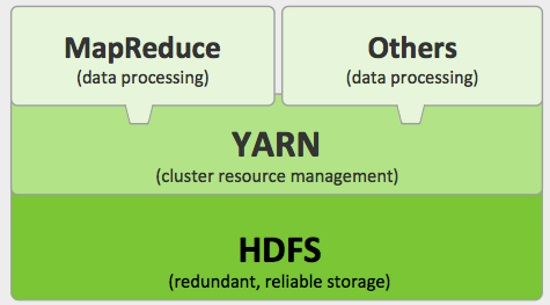
\includegraphics[width=\linewidth]{architecture.jpg}
    \caption{Architettura}
    \label{fig:architecture}
  \end{center}
\end{figure}
\subsection{HDFS}
HDFS è il filesystem distribuito che utilizza il framework Hadoop per processare i dati. I punti di forza su cui si basa sono i seguenti:
\begin{description}
  \item[Memorizzazione di grandi file:] Dove in questo contesto indichiamo file che sono centinaia di megabyte, gigabyte o terabyte.
  \item[Accesso dati:] HDFS è costruito intorno all'idea che il migiore pattern per processare i dati è "una scrittura e tante letture". Un dataset è tipicamente generato o copiato da una sorgente e successivamente varie analisi sono effettuate sul dataset nel tempo. Ogni analisi richiede grandi porzioni se non l'intero dataset quindi il tempo per leggere l'intero dataset è più importante della latenza di leggere il primo record.
  \item[Commodity Hardware:]Hadoop non richiede hardware costoso. È strutturato per essere eseguito su cluster basato su commodity hardware (hardware comunemente disponibile che può essere ottenuto da diversi fornitori).
\end{description}
\subsubsection{Blocchi}
Sappiamo che i dischi hanno una \textit{block-size} che rappresenta l'ammontare minimo di dati che possono leggere o scrivere. Di solito la grandezza di questi blocchi è nell'ordine dei kilobyte ma in HDFS questa grandezza è pari a 128MB e una caratteristica importante è che file più piccoli del blocco non occupano quest'ultimo interamente (ad esempio se avessimo un file da 1MB esso utilizzerà 1MB di disco e non 128). I motivi per cui questi blocchi sono così grandi sono vari: il primo è per minimizzare i tempi di ricerca nel disco, il secondo è che avere questa astrazione a blocchi, permette di memorizzare file più grandi di un singolo disco e inoltre semplifica la gestione della memorizzazione dei dati in quanto avere blocchi di taglia fissa permette di calcolare facilmente quanti ne possono essere memorizzati du di un disco ed elimina la gestione dei metadati (che vengono gestiti a parte).
\subsubsection{Namenode e Datanode}
Un cluster HDFS ha due tipologie di nodi che seguono il paradigma master-slave: un \textbf{namenode} (master) ed un numero di \textbf{datanode} (slave). Il primo gestisce il namespace del filesystem e i metadati per tutte le direcrory e i file e memorizza queste informazioni sul proprio disco locale oltre a conoscere la locazione dei blocchi di ogni file. I secondi invece memorizzano e processano i dati riportando periodicamente al namenode quale lista di blocchi memorizzano. La perdita del namenode comporta l'inutilizzabilità del filesystem ed è quindi importante avere un \textit{secondary-namenode} che periodicamente si sincronizza con il primary per fungere da backup in caso di guasti o malfunzionamento.
\subsection{Yarn}
\textbf{Apache YARN} (Yet Another Resource Negotiator) è il sistema della gestione delle risorse in Hadoop. Introdotto dalla versione 2 di Hadoop ha migliorato di molto le prestazioni del framework. Yarn fornisce i suoi servizi attraverso due processi manager, un \textit{resource-manager} (uno per cluster) per gestire l'uso delle risorse e un \textit{node-manager} che è eseguito su tutti i nodi nel cluster per lanciare e monitorare i container (Esegue i task con un insieme ristretto di risorse). Per eseguire un applicativo su YARN il client contatta il resource-manager e gli chiede di lanciare un \textit{application-master}. Quello che fa l'application master dipende dal tipo di applicazione: può semplicemente eseguire il job sul proprio container o richiederne altri per distribuire la computazione.
\begin{figure}
  \begin{center}
    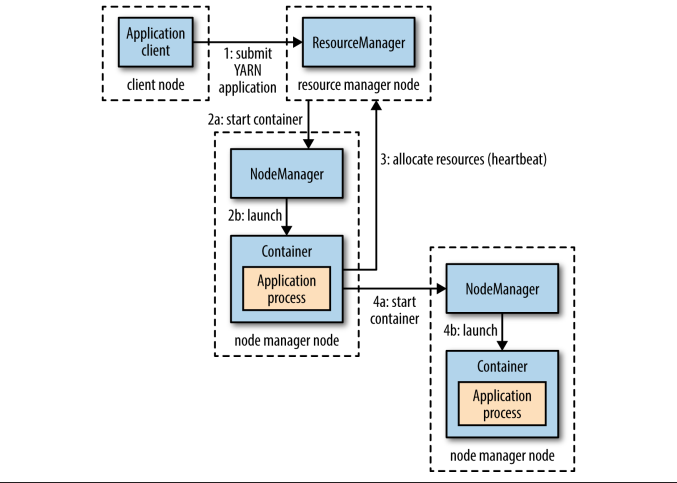
\includegraphics[width=\linewidth]{yarn.png}
    \caption{Esempio di Esecuzione di YARN}
    \label{fig:yarn}
  \end{center}
\end{figure}
\subsection{Paradigma Map-Reduce}
Map-Reduce è un modello di programmazione per processare i dati. I programmi Map-Reduce sono inerentemente paralleli, così da permettere di fare analisi di dati in larga scala se a disposizione di abbastanza macchine, in particolare questo modello funziona al meglio con dataset di grandi dimensioni. Hadoop è in grado di eseguire programmi Map-Reduce scritti in vari linguaggi tra cui Java, Python e Ruby e il suo funzionamento suddivide il lavoro in due fasi: la fase di map e di reduce. Ogni fase ha delle coppie chiave-valore come input e output, i cui tipi potrebbero essere scelti dal programmatore. Il programmatore specifica anche due funzioni: la funzione di map e la funzione di reduce. Nello specifico Map prende in input una coppia \textit{<K,V>} e restituisce in output una lista di coppie intermedie \textit{<K',V'>} mentre Reduce acquisisce in input una lista di coppie intermedie \textit{<K,V> } con la stessa chiave e restituisce in output una lista di coppie \textit{<K',V'>}. Il paradigma Map-Reduce fornisce oltre alle suddette funzioni, anche parallelizzazione, distribuzione automatica, fault tolerance, schedulazione I/O, status e monitoring. Un programma costruito secondo questo modello divide i dati in input tramite la libreria MapReduce ed eseguiti tramite varie istanze del programma su un cluster di macchine. Una delle istanze, il master assegna i task alle altre macchine, gli slave (o worker).
\subsubsection{Map}
In questa fase un worker legge il blocco di input assegnato, dopodiché estrae da esso le coppie \textit{<K,V>} e le passa una alla volta alla funzione \textit{map()}. La funzione \textit{map()} a sua volta produce delle coppie \textit{<K',V'>}. Per creare un mapper in Java è necessario che una classe estenda la classe Mapper che presenta la seguente firma:
\begin{lstlisting}
public class Mapper<KEYIN, VALUEIN, KEYOUT, VALUEOUT> {
  protected void map(KEYIN key, VALUEIN value, Context context) throws IOException, InterruptedException {
    //method body here
  }
}
\end{lstlisting}
Nel corpo del metodo \textit{map} è possibile inserire il proprio algoritmo per trasformare l'input nella maniera che si desidera da mandare al reduce con il metodo \textit{write} dell'instanza dell'oggetto di tipo \textit{Context}. Questo oggetto rappresenta il mezzo tramite il quale i Mapper e i Reducer interagiscono con il resto dell'ecosistema di Hadoop ed include informazioni fondamentali come ad esempio la configurazione dei job.
\subsubsection{Reduce}
Il master a questo punto assegna ad un worker un task di tipo reduce indicandogli una regione di dati da "ridurre". Un task reduce consiste nel prendere tutte le coppie \textit{<K,V>} raggruppate in modo che le chiavi siano uniche. Ogni gruppo viene passato quindi alla funzione \textit{reduce()}. In Java un reducer si crea estendendo la classe Reducer che ha la seguente firma:
\begin{lstlisting}
public class Reducer<KEYIN, VALUEIN, KEYOUT, VALUEOUT> {
  protected void reduce(KEYIN key, Iterable<VALUEIN> values, Context context) throws IOException, InterruptedException {
    //method body here
  }
}
\end{lstlisting}
Nel corpo del metodo \textit{reduce} è possibile inserire il proprio algoritmo per eseguire l'aggregazione degli output dei task map. Anche il reducer fa uso dell'oggetto \textit{Context} e del metodo \textit{write} per scrivere l'output prodotto. Sia Mapper che Reducer implementano due funzioni di hook chiamate all'inizio e alla fine di ogni task un'unica volta e sono rispettivamente il metodo \textit{setup()} e \textit{cleanup()} e sono utili quando c'è da effettuare un insieme di operazioni inizializzazione o di pulizia.
\subsubsection{Splitter}
Lo Splitter è quella componente che ha il compito di prendere l’intero input e di dividerlo in \textbf{InputSplit}, che verranno poi inviati ai vari map task. La mappatura \textit{< K, V >} degli InputSplit viene definita dalla classe InputFormat implementata. Hadoop mette a disposizione diverse implementazioni di InputFormat, ciononostante è possibile, ovviamente, definirne uno proprio da utilizzare durante la computazione implementando l’interfaccia \textit{InputFormat}. È da sottolineare il fatto che non si deve confondere l’InputSplit con il blocco utilizzato dall’HDFS. I due "blocchi" non necessariamente corrispondono. Possono infatti verificarsi dei casi in cui l’InputSplit utilizza dati presenti in più blocchi, causando un leggero overhead del sistema. Il framework Hadoop mette a disposizione diversi splitter oltre a poterni creare di nuovi creando una nuova classe che estenda la classe \textit{InputSplit}.
\begin{lstlisting}
public abstract class InputSplit {
  public abstract long getLength() throws IOException, InterruptedException;
  public abstract String[] getLocations() throws IOException, InterruptedException;
}
\end{lstlisting}
Questa classe non contiene alcun tipo di dato ma solo i riferimenti dell'ubicazione e della lunghezza di questi ultimi infatti questa classe è d'aiuto alle classi \textit{InputFormat} e \textit{RecordReader} le quali sono responsabili di recuperare e leggere i dati in maniera efficiente per i MapReduce Task.
\subsubsection{Partitioner}
I Partitioner sono responsabili di dividere le coppie \textit{<K, V>} intermedie generate dai MapTask ai vari Reducer per la funzione di Reduce. Per dividere in maniera equa i compiti ai Reducer, i partitioner usano una funzione di hash sulla chiave: $reducer = hash(K) \bmod n$. Implementare un partitioner personalizzato in Java richiede estendere la classe \textit{Partitioner} che presenta la seguente interfaccia:
\begin{lstlisting}
public abstract class Partitioner<KEY, VALUE> {
  public abstract int getPartition(KEY key, VALUE value, int numPartitions);
}
\end{lstlisting}
Di default hadoop utilizza un \textit{HashPartitioner} il cui funzionamento è stato riportato poc'anzi.
\subsubsection{Combiner}
I Combiner permettono l'aggregazione in locale prima della fasi di shuffle permettendo così di compattare l'input prima di essere spedito sulla rete ai reducer. In Java un Combiner deve estendere la classe Reducer, opera su ogni output del map task e le coppie chiavi-valore in output devono corrispondere a quelle del Reduce.
\subsubsection{Shuffle e Sort}
Map-Reduce garantisce che l'input ad ogni reducer sia ordinato per chiave. Il processo con il quale il sistema esegue il sort, e trasferisce gli output del map ai reducer come input, è conosciuto come shuffle.
\section{Come funziona un Job Map Reduce}
A grandi linee possiamo riassumere un'esecuzione di MapReduce nei seguenti punti:
\begin{enumerate}
  \item Lettura dei dati;
  \item Inputsplitting;
  \item Mapping;
  \item Combining; 
  \item Partitioning, Shuffling e Sorting;
  \item Reducing;
\end{enumerate}
È possibile eseguire un job MapReduce con una singola chiamata al metodo \textit{submit()} di un oggetto Job. Questa chiamata al metodo cela molta computazione ed è opportuno capire quali sono i passi compiuti da Hadoop  per eseguire un job. L'intero processo comprende, da una vista ad alto livello, cinque entità indipendenti:
\begin{enumerate}
  \item Il client, che sottomette il job MapReduce;
  \item Il resource maanger YARN, che coordina e monitora i container di calcolo sulle macchine del cluster;
  \item I node manager YARN, che lanciano e monitorano i container di calcolo sulle macchine del cluster;
  \item L'application master MapReduce, che coordina i task che eseguono il job MapReduce. L'application master e i task MapReduce sono eseguiti in container che sono schedulati dal resource manager e gestiti dai node manager;
  \item Il distributed filesystem (HDFS), che è usato per condivedere file tra altre entità.
\end{enumerate}
\begin{figure}
  \begin{center}
    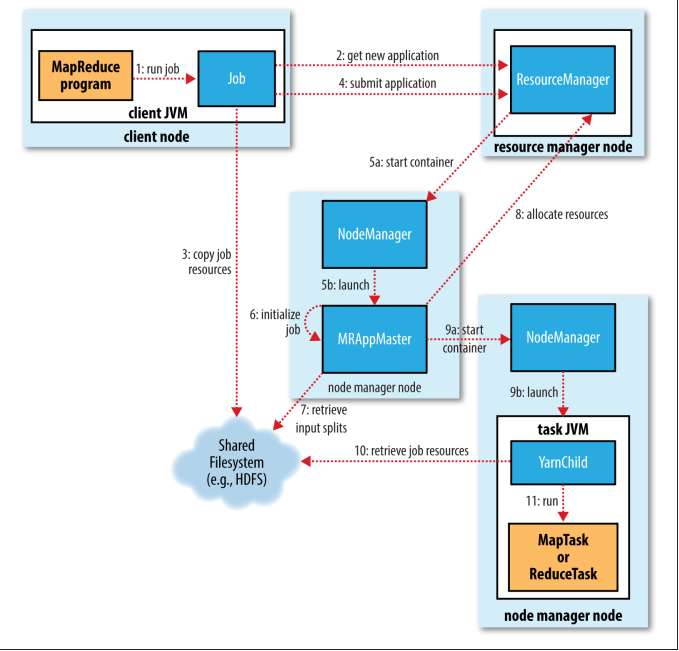
\includegraphics[width=\linewidth]{mapReduceJob.png}
    \caption{L'esecuzione di un job MapReduce di Hadoop}
    \label{fig:job}
  \end{center}
\end{figure}
\subsection{Sottomissione del Job}
Il metodo \textit{submit()}, effettuato su un Job, crea un'istanza interna JobSubmitter e chiama \textit{submitJobInterval()} su di esso. Avendo sottomesso il job, \textit{waitForCompletion()} sonda il progresso di job e riporta il progresso alla console se è cambiato dall'utlimo report. Quando un job è completato con successo, i risultati sono mostrati in output, altrimenti, l'errore che ha causato il fail del job è loggato in console.
\subsection{Inizializzazione del job}
Quando il resource maanger riceve una chiamata al metodo \textit{submitApplication()}, consegna la richiesta allo YARN scheduler. Lo scheduler alloca un container, e il resource manager lancia il processo dell'application master, sotto la gestione del node manager. L'application master per i job MapReduce è un'applicazione Java la cui classe principale è \textit{MRAppMaster}. Esso inizializza il job creando un numero di oggetti bookkeping per tenere traccia del progresso del job, dato che riceverà report sul progresso e sul completamento dai task. Successivamente, recupera gli input split calcolati nel client dal filesystem condiviso. Quindi crea un oggetto map task per ogni split, così come un numero di oggetti reduce task determinato dalla proprietà \textit{mapreduce.job.reduces}. I task a questo punto ricevono l'ID. L'application master deve anche decidere come eseguire i task che costituiscono il job MapReduce e se il job è piccolo, l'application master potrebbe scegliere di eseguire i task nella sua stessa JVM. Infine, prima che qualsiasi task venga eseguito, l'application master chiama il metodo \textit{setupJob()} sull'OutputCommitter. Per il FileOutputCommitter, che è di default, creerà la directory di output finale per il job e lo spazio di lavoro temporaneo per il task di output.
\subsection{Esecuzione del Task}
Una volta che a un task sono state assegnate risorse per un container su un particolare nodo dallo scheduler del resource manager, l'application master avvia il container contattando il node manager. Il task è eseguito da un'applicazione Java la cui main class è YarnChild. Prima che possa eseguire il task, localizza le risorse di cui il task ha bisogno, inclusa la configurazione del job e un JAR file, e qualsiasi file dalla cache distribuita. Alla fine, esegue il map o il reduce task. \\
Il YarnChild è eseguito in una JVM dedicata, così che qualsiasi bug nel map user-defined e le funzioni reduce (o anche in YarnChild) non influenzino il node manager, causandone il crash.\newline
Ogni task può eseguire azioni di setup e commit, che sono eseguite sulla stessa JVM come il task stesso e sono determinate dall'OutputCommitter per il job. Per i job file-based, il commit sposta l'output del task da una locazione temporanea alla sua locazione finale. Il protocollo di commit assicura che quando l'esecuzione speculativa è abilitata, solo di uno dei task duplicati verrà fatto il commit e gli altri saranno abortiti.
\subsection{Completamento di un job}
Quando il master application riceve una notifica che l'ultimo task per un job è completo, cambia lo stato per il job a "successful" e quindi, quando il Job sonda lo stato, apprende che il job è stato completato con successo e stampa un messaggio per dirlo all'utente e ritorna dal metodo \textit{waitForCompletion()}. Le statistiche e i counter di un Job sono stampati su console a questo punto. L'application master invia anche una job notification HTTP se è configurato per farlo. Questo può essere configurato dai client che vogliono ricevere callback, tramite la proprietà \textit{mapreduce.job.end-notification.url}. Infine, al completamento di un job, l'application master e i task container puliscono il loro working state (così l'output intermedio è cancellato), e il metodo \textit{commitJob()} di OutputCommitter è chiamato. Informazioni del Job sono registrate dal job history server per consentire successive interrogazioni dagli utenti se desiderato.
\subsection{Shuffle e Sort}
Lo shuffle è un'area del codebase dove raffinamenti e miglioramenti sono continuamente effettuati, costituisce il cuore di MapReduce ed è qui che avviene la "magia".
\subsubsection{Il lato Map}
Quando la funzione \textit{map} comincia a produrre output, questo non è semplicemente scritto su disco. Il processo è più complesso, e prende vantaggi dalla bufferizzazione delle scritture in memoria ed effettua qualche preordinamento per ragioni di efficienza. Ogni map task ha un buffer di memoria circolare su cui scrive l'output. Quando i contenuti del buffer raggiungono un certo limite di taglia, un thread in background comincerà a fare \textbf{spill} dei contenuti su disco, ovvero sposta i dati  dalla memoria RAM a quella del disco. I map output continueranno a essere scritti sul buffer fino a quando non avviene lo spill, ma se il buffer nel frattempo si riempie, il map si bloccherà sino al completamento dello spill. Gli spill sono scritti in round robin alle cartelle specificate dalla proprietà \textbf{mapreduce.cluster.local.dir}, in una sottocartella specifica al job. Prima che scriva sul disco, il thread prima divide i dati in partizioni corrispondenti ai reducer a cui saranno inviati alla fine e in ogni partizione, il thread in background esegue un ordinamento per chiave in memoria, e se c'è una funzione di combiner, è eseguito sull'output dell'ordinamento. L'esecuzione della funzione di combiner fa ottenere un map output più compatto, quindi ci sono meno dati da scrivere sul disco locale e da trasferire al reducer. Ogni volta che il buffer di memoria raggiunge il limite di spill, un nuovo spill file viene creato, così dopo che il map task ha scritto il suo ultimo record di output, ci potrebbero essere vari spill file. Prima che il task termini, si effettua il merge dei spill file in un singolo file di output partizionato ed ordinato. La proprietà di configurazione \textbf{mapreduce.task.io.sort.factor} controlla il massimo numero di stream di cui fare il merge alla volta; il valore di default è 10. Se ci sono almeno tre spill file, il combiner è eseguito di nuovo prima che il file di output sia scritto. I combiner potrebbero essere eseguiti ripetutamente sugli input senza influire sul risultato finale. Se ci sono solo uno o due spill, la riduzione potenziale nella taglia del map output non vale l'overhead dell'invocazione del combiner, quindi non è eseguita di nuovo per questo map output. È spesso una buona idea comprimere il map output alla scrittura sul disco, perchè fare ciò rende più veloce la scrittura su disco, risparmia spazio sul disco, e riduce la quantità di dati da trasferire al reducer. Di default, l'output non è compresso, ma è facile abilitare quest'impostazione settandola con \textbf{mapreduce.map.output.compress.codec}. Le partizioni del file di output sono rese disponibili ai reducer con HTTP. Il massimo numero di worker thread usato per servire le partizioni del file è controllato dalla proprietà \textbf{mapreduce.shuffle.max.threads}.
\subsubsection{Il lato Reduce} 
Il file di map output si trova sul disco locale della macchina che ha eseguito il map task (è da notare che nonostante i map output siano sempre scritti sul disco locale, i reduce output potrebbero non esserlo), ma ora è necessario per la macchina che sta per eseguire il reduce task per perchè ha bisogno del map output per la sua specifica partizione da vari map task nel cluster. I map task potrebbero finire in tempi diversi, quindi il reduce task comincia a copiare i loro output non appena ognuno è stato completato. Questa è conosciuta come fase di copia del reduce task. Il reduce task ha un piccolo numero di thread di copia così che possa prendere i map output in parallelo. Di default ci sono cinque thread, ma questo numero può essere cambiato settando la proprietà \textit{mapreduce.reduce.shuffle.parallelcopies}. Al completamento dei map task, essi notifcano il loro application master secondo il meccanismo di heartbeat. Perciò, per un dato job, l'application master conosce l'associazione tra i map output e gli host. Un thread nel reducer periodicamente chiede al master gli host del map output fino a quando non li ha recuperati tutti. Gli host cancellano i map output dal disco non appena il primo reducer li ha recuperati ma, siccome il reducer potrebbe successivamente fallire, aspettano fino a quando non gli viene detto di rimuoverli dall'application master, il che avviene dopo che il job è stato completato. I map output sono copiati nella memoria della JVM del reduce task se sono abbastanza piccoli (la taglia del buffer è controllata da \textit{mapreduce.reduce.shuffle.input.buffer.percent}, che specifica la proporzione dell'heap da usare per questo scopo); altrimenti, sono copiati su disco. Quando il buffer in memoria raggiunge il limite di taglia o raggiunge un numero limite di map output, ne viene effettuato il merge e lo spill su disco. Se un combiner è specificato, sarà eseguito durante il merge per ridurre la quantità di dati scritti su disco. All'accumularsi delle copie su dico, un thread in background ne fa il merge in file più grandi e ordinati così si risparmia tempo effettuando il merge in un secondo momento. Si nota che qualsiasi map output che è stato compresso (dal map task) deve essere decompresso in memoria per eseguire il loro merge. Quando tutti i map output sono stati copiati, il reduce task passa alla fase di ordinamento (che dovrebbe essere propriamente chiamata fase di merge, siccome l'ordinamento è stato effettuato nel lato map), che fa il merge dei map output, mantenendo il loro ordine di suddivisione. Ciò avviene in fasi: per esempio, se ci fossero 50 map output e il fattore di merge fosse 10, ci sarebbero cinque fasi dove ogni fase farebbe il merge di 10 file in 1, così alla fine ci sarebbero 5 file intermedi.
Piuttosto che avere una fase finale che fa il merge di questi cinque file in un unico file ordinato, il merge salva un trip su disco fornendo direttamente la funzione di reduce in quella che è l'ultima fase: la fase di reduce. Il merge finale può venire da un misto di segmenti in memoria e su disco. Il numero di file di cui si fa il merge in ogni fase è in verità più sottile di quanto quest'esempio suggerisca. Lo scopo è fare il merge del numero minimo di file da ricevere al fattore di merge per il passo finale. Quindi se ci fossero 40 file, il merge non farebbe il merge di 10 file in ognuna delle quattro fasi per ottenere 4 file. Invece, la prima fase farebbe il merge di solo 4 file, e le seguenti tre fasi farebbero il merge i 10 file. I 4 file ottenuti con il merge e i 6 file (di cui non è stato fatto ancora il merge) fanno un totale di 10 file per la fase finale.
\begin{figure}
  \begin{center}
    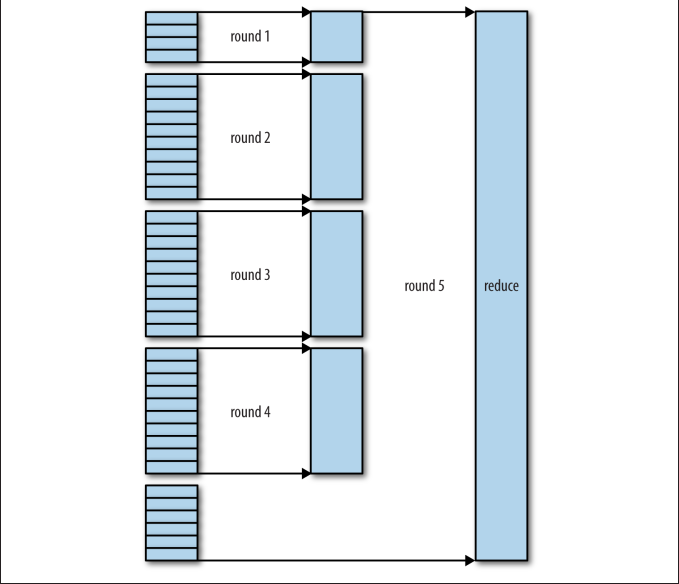
\includegraphics[width=\linewidth, scale=0.3]{effmerge.png}
    \caption{Merge efficiente per 40 segmenti di file con un fattore di merge pari a 10}
    \label{fig:merge}
  \end{center}
\end{figure}
Il numero di fasi rimane invariato; è solo un'ottimizzazione per minimizzare la quantità di dati scritti su disco, dato che il passo finale fa il merge direttamente nella reduce.
Durante la fase di reduce, la funzione di reduce è invocata per ogni chiave nell'output ordinato. L'output di questa fase è scritto direttamente sul filesystem di output, tipicamente HDFS. Nel caso di HDFS, dato che il node manager sta anche eseguendo un datanode, il primo blocco di replica sarà scritto sul disco locale.
\newpage
\section{Progetti Correlati}
la fondazione Apache ha creato un insieme di progetti che si appoggiano su Hadoop, tutti quanti di ottimo successo, e che si focalizzano su particolari casi d'uso:
\begin{description}
  \item[Apache Avro]:È un sistema di serializzazione dei dati utilizzato per poter sostituire quello che viene comunemente definito il problema maggiore di Haddop ovvero la non portabilità dei dati serializzati tramite i \textit{Writable}. I dati vengono descritti tramite l'ausilio di schemi scritti in JSON oppure tramite \textit{L'Avro IDL}. Un'altra caratteristica è che questi file possono essere splittabili e compressi e quindi utili per poter essere utilizzati dal MapReduce ed esendo indipendenti dal linguaggio, possono essere consumati anche utilizzando altri linguaggi di programmazione che non siano Java.
  \item[Apache Parquet:] È un formato di storage a colonne capace di memorizzare in maniera efficiente dati innestati. Memorizzare a colonne può essere molto vantaggioso in termini di spazio e di efficienza: nel primo caso lo storage è più efficiente di quello a righe perchè i dati sono "simili" e facili da codificare (ad esempio se si volesse memorizzare un timestamp si portebbe memorizzare il primo valore e nelle colonne succesive solamente i delta di tempo passati), nel secondo caso un query engine può saltare le colonne che non sono utili alla query. Questo formato è stato sviluppato da Twitter e Cloudera (uno dei piàù importanti fornitori di ambienti hadoop) utilizzanod tecninche innovative per memorizzare file in formato colonne rendendo minimi gli overhead. Anche questo fomrmato ècompatibile con MapReduce.
  \item[Apache Flume:] Ci sono molti sistemi che non fanno uso dell'HDFS per processare i dati ma allo stesso tempo hanno bisogno del MapReduce per processarli. Apache Flume cerca di andare incotro a questa esigenza, ed ha creato un ecosistema per processare enormi moli di dati event-based per poi mandarli ad Hadoop. Un esempio possono essere il log file di un web server e in questo caso Flume automatizza il processo di aggregazione dei file e spostamento sull'HDFS in maniera trasparente. L'idea è quella di lanciare dei processi Java (agent) in distribuito che collezionano i dati, li aggregano e li memorizzano nella sua destinazione finale.
  \item[Apache Sqoop:] A volte può succedere che il dataset su cui debba lavorare un job MapReduce, sia memorizzato in maniera struttrata all'interno di store strutturati come ad esempio un RDBMS. Sqoop risolve questo problema estraendo questi dati passandoli così ad Hadoop per effettuare le sue analisi.
  \item[Apache Pig:] Basato su MapReduce, si pone ad un livello di astrazione ancora più alto, permettendo di manipolare dati più complessi ed effettuando operazioni che non sono possibile normalmente su Hadoop (come ad esempio le join tra i dati). È formato da due componenti: il linguaggio utilizzato per lavorare sul flusso dei dati chiamato \textbf{Pig Latin} e l'ambiente di esecuzione che può essere centralizzato o distribuito al di sopra di un cluster Hadoop. È stato reato da Yahoo in risposta alle loro esigenze di effettuare mining su enrìormi moli di dati. 
  \item[Apache Hive:] È un framework sviluppato per effettuare data warehousing con Hadoop. Ideato da Facebook per permettere a chi ha una buona padroanza con SQL di eseguire query su enormi volumi di dati e ad oggi riscuote un buon successo perchè utilizzato da molte organizzazioni per scopi di tutti i tipi.
  \item[Apache Crunch:] È un insieme di API ad alto livello per produrre pipeline di MapReduce job. Il vantaggio principale che offre è che utilizza come tipi di dato quelli di Java, un insieme di operazioni di trasformazione dei dati già pronte all'utilizzo.
  \item[Apache Spark:] Anch'esso serve per processare moli di dati ma a differenza degli ambienti precedenti, non si appoggia su MapReduce ma utilizza un suo runtime  però può essere integrato con YARN e HDFS. Spark è conosciuto per la sua abilità di mantenere grossi dataset in memoria tra i diversi job e questo approccio funziona bene su algoritmi di tipo iterativo e su analisi interattive.
  \item[Apache HBase:] È un database distribuito orientato a colonne costruito al di sopra di HDFS. Il suo uso comune è per costruire \textbf{webtable}.
  \item[Apache Zookeeper:] È un servizio di coordinamento che permette di costruire applicazioni distribuite riducendo al minimo le failure.
\end{description}
